% GNUPLOT: LaTeX picture with Postscript
\begingroup
  \makeatletter
  \providecommand\color[2][]{%
    \GenericError{(gnuplot) \space\space\space\@spaces}{%
      Package color not loaded in conjunction with
      terminal option `colourtext'%
    }{See the gnuplot documentation for explanation.%
    }{Either use 'blacktext' in gnuplot or load the package
      color.sty in LaTeX.}%
    \renewcommand\color[2][]{}%
  }%
  \providecommand\includegraphics[2][]{%
    \GenericError{(gnuplot) \space\space\space\@spaces}{%
      Package graphicx or graphics not loaded%
    }{See the gnuplot documentation for explanation.%
    }{The gnuplot epslatex terminal needs graphicx.sty or graphics.sty.}%
    \renewcommand\includegraphics[2][]{}%
  }%
  \providecommand\rotatebox[2]{#2}%
  \@ifundefined{ifGPcolor}{%
    \newif\ifGPcolor
    \GPcolorfalse
  }{}%
  \@ifundefined{ifGPblacktext}{%
    \newif\ifGPblacktext
    \GPblacktexttrue
  }{}%
  % define a \g@addto@macro without @ in the name:
  \let\gplgaddtomacro\g@addto@macro
  % define empty templates for all commands taking text:
  \gdef\gplbacktext{}%
  \gdef\gplfronttext{}%
  \makeatother
  \ifGPblacktext
    % no textcolor at all
    \def\colorrgb#1{}%
    \def\colorgray#1{}%
  \else
    % gray or color?
    \ifGPcolor
      \def\colorrgb#1{\color[rgb]{#1}}%
      \def\colorgray#1{\color[gray]{#1}}%
      \expandafter\def\csname LTw\endcsname{\color{white}}%
      \expandafter\def\csname LTb\endcsname{\color{black}}%
      \expandafter\def\csname LTa\endcsname{\color{black}}%
      \expandafter\def\csname LT0\endcsname{\color[rgb]{1,0,0}}%
      \expandafter\def\csname LT1\endcsname{\color[rgb]{0,1,0}}%
      \expandafter\def\csname LT2\endcsname{\color[rgb]{0,0,1}}%
      \expandafter\def\csname LT3\endcsname{\color[rgb]{1,0,1}}%
      \expandafter\def\csname LT4\endcsname{\color[rgb]{0,1,1}}%
      \expandafter\def\csname LT5\endcsname{\color[rgb]{1,1,0}}%
      \expandafter\def\csname LT6\endcsname{\color[rgb]{0,0,0}}%
      \expandafter\def\csname LT7\endcsname{\color[rgb]{1,0.3,0}}%
      \expandafter\def\csname LT8\endcsname{\color[rgb]{0.5,0.5,0.5}}%
    \else
      % gray
      \def\colorrgb#1{\color{black}}%
      \def\colorgray#1{\color[gray]{#1}}%
      \expandafter\def\csname LTw\endcsname{\color{white}}%
      \expandafter\def\csname LTb\endcsname{\color{black}}%
      \expandafter\def\csname LTa\endcsname{\color{black}}%
      \expandafter\def\csname LT0\endcsname{\color{black}}%
      \expandafter\def\csname LT1\endcsname{\color{black}}%
      \expandafter\def\csname LT2\endcsname{\color{black}}%
      \expandafter\def\csname LT3\endcsname{\color{black}}%
      \expandafter\def\csname LT4\endcsname{\color{black}}%
      \expandafter\def\csname LT5\endcsname{\color{black}}%
      \expandafter\def\csname LT6\endcsname{\color{black}}%
      \expandafter\def\csname LT7\endcsname{\color{black}}%
      \expandafter\def\csname LT8\endcsname{\color{black}}%
    \fi
  \fi
    \setlength{\unitlength}{0.0500bp}%
    \ifx\gptboxheight\undefined%
      \newlength{\gptboxheight}%
      \newlength{\gptboxwidth}%
      \newsavebox{\gptboxtext}%
    \fi%
    \setlength{\fboxrule}{0.5pt}%
    \setlength{\fboxsep}{1pt}%
\begin{picture}(9360.00,7200.00)%
    \gplgaddtomacro\gplbacktext{%
      \colorrgb{0.50,0.50,0.50}%
      \put(1240,1722){\makebox(0,0){\strut{}$-2$}}%
      \colorrgb{0.50,0.50,0.50}%
      \put(1634,1609){\makebox(0,0){\strut{}$-1.5$}}%
      \colorrgb{0.50,0.50,0.50}%
      \put(2027,1496){\makebox(0,0){\strut{}$-1$}}%
      \colorrgb{0.50,0.50,0.50}%
      \put(2421,1383){\makebox(0,0){\strut{}$-0.5$}}%
      \colorrgb{0.50,0.50,0.50}%
      \put(2815,1270){\makebox(0,0){\strut{}$0$}}%
      \colorrgb{0.50,0.50,0.50}%
      \put(3208,1158){\makebox(0,0){\strut{}$0.5$}}%
      \colorrgb{0.50,0.50,0.50}%
      \put(3602,1045){\makebox(0,0){\strut{}$1$}}%
      \colorrgb{0.50,0.50,0.50}%
      \put(3995,932){\makebox(0,0){\strut{}$1.5$}}%
      \colorrgb{0.50,0.50,0.50}%
      \put(4389,819){\makebox(0,0){\strut{}$2$}}%
      \csname LTb\endcsname%
      \put(2427,975){\makebox(0,0){\strut{}x [m]}}%
      \colorrgb{0.50,0.50,0.50}%
      \put(4569,860){\makebox(0,0){\strut{}$-2$}}%
      \colorrgb{0.50,0.50,0.50}%
      \put(4797,1055){\makebox(0,0){\strut{}$-1.5$}}%
      \colorrgb{0.50,0.50,0.50}%
      \put(5024,1251){\makebox(0,0){\strut{}$-1$}}%
      \colorrgb{0.50,0.50,0.50}%
      \put(5251,1446){\makebox(0,0){\strut{}$-0.5$}}%
      \colorrgb{0.50,0.50,0.50}%
      \put(5479,1641){\makebox(0,0){\strut{}$0$}}%
      \colorrgb{0.50,0.50,0.50}%
      \put(5706,1837){\makebox(0,0){\strut{}$0.5$}}%
      \colorrgb{0.50,0.50,0.50}%
      \put(5933,2032){\makebox(0,0){\strut{}$1$}}%
      \colorrgb{0.50,0.50,0.50}%
      \put(6161,2228){\makebox(0,0){\strut{}$1.5$}}%
      \colorrgb{0.50,0.50,0.50}%
      \put(6388,2423){\makebox(0,0){\strut{}$2$}}%
      \csname LTb\endcsname%
      \put(6152,1470){\makebox(0,0){\strut{}y [m]}}%
      \colorrgb{0.50,0.50,0.50}%
      \put(1180,1817){\makebox(0,0)[r]{\strut{}$-2$}}%
      \colorrgb{0.50,0.50,0.50}%
      \put(1180,2208){\makebox(0,0)[r]{\strut{}$-1.5$}}%
      \colorrgb{0.50,0.50,0.50}%
      \put(1180,2599){\makebox(0,0)[r]{\strut{}$-1$}}%
      \colorrgb{0.50,0.50,0.50}%
      \put(1180,2989){\makebox(0,0)[r]{\strut{}$-0.5$}}%
      \colorrgb{0.50,0.50,0.50}%
      \put(1180,3380){\makebox(0,0)[r]{\strut{}$0$}}%
      \colorrgb{0.50,0.50,0.50}%
      \put(1180,3770){\makebox(0,0)[r]{\strut{}$0.5$}}%
      \colorrgb{0.50,0.50,0.50}%
      \put(1180,4161){\makebox(0,0)[r]{\strut{}$1$}}%
      \colorrgb{0.50,0.50,0.50}%
      \put(1180,4552){\makebox(0,0)[r]{\strut{}$1.5$}}%
      \colorrgb{0.50,0.50,0.50}%
      \put(1180,4942){\makebox(0,0)[r]{\strut{}$2$}}%
      \csname LTb\endcsname%
      \put(382,3380){\makebox(0,0){\strut{}z [m]}}%
      \put(6522,4854){\makebox(0,0)[l]{\strut{}Ausschnitt (vergrößert)}}%
    }%
    \gplgaddtomacro\gplfronttext{%
      \csname LTb\endcsname%
      \put(5725,6696){\makebox(0,0)[r]{\strut{}getestete Positionen (für r=1.4m)}}%
      \csname LTb\endcsname%
      \put(5725,6696){\makebox(0,0)[r]{\strut{}getestete Positionen (für r=1.4m)}}%
    }%
    \gplgaddtomacro\gplbacktext{%
    }%
    \gplgaddtomacro\gplfronttext{%
    }%
    \gplbacktext
    \put(0,0){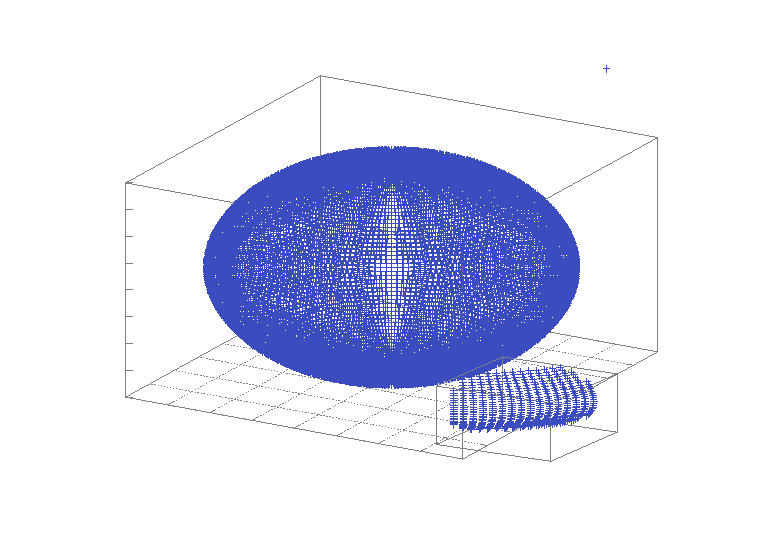
\includegraphics{img/tested_positions_zoom}}%
    \gplfronttext
  \end{picture}%
\endgroup
